\subsection{UC10 - Nascondi applicazione}
\begin{figure}[H]
    \centering
    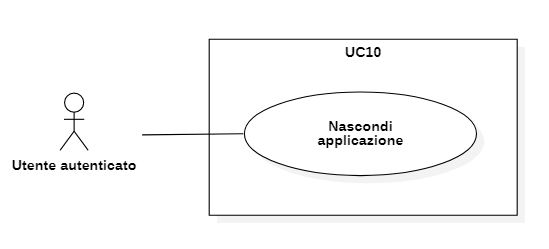
\includegraphics[scale = 0.7]{components/img/UC10.png}
    \caption{UC10 - Nascondi applicazione}
\end{figure}
\begin{itemize}
\item \textbf{Attore Primario:} Utente autenticato;
\item \textbf{Precondizione:} L'applicazione è mostrata a schermo;
\item \textbf{Postcondizione:} L'applicazione viene mostrata nell'area di notifica;
\item \textbf{Scenario principale:}
    \begin{enumerate}
    \item L'utente visualizza l'applicazione a tutto schermo;
    \item L'utente chiude l'applicazione.
    \end{enumerate}
\end{itemize}